\begin{frame}
\frametitle{子图并排展示}
\framesubtitle{利用 subfig 宏包实现}

\begin{figure}
\centering
\subfloat[校园风光]{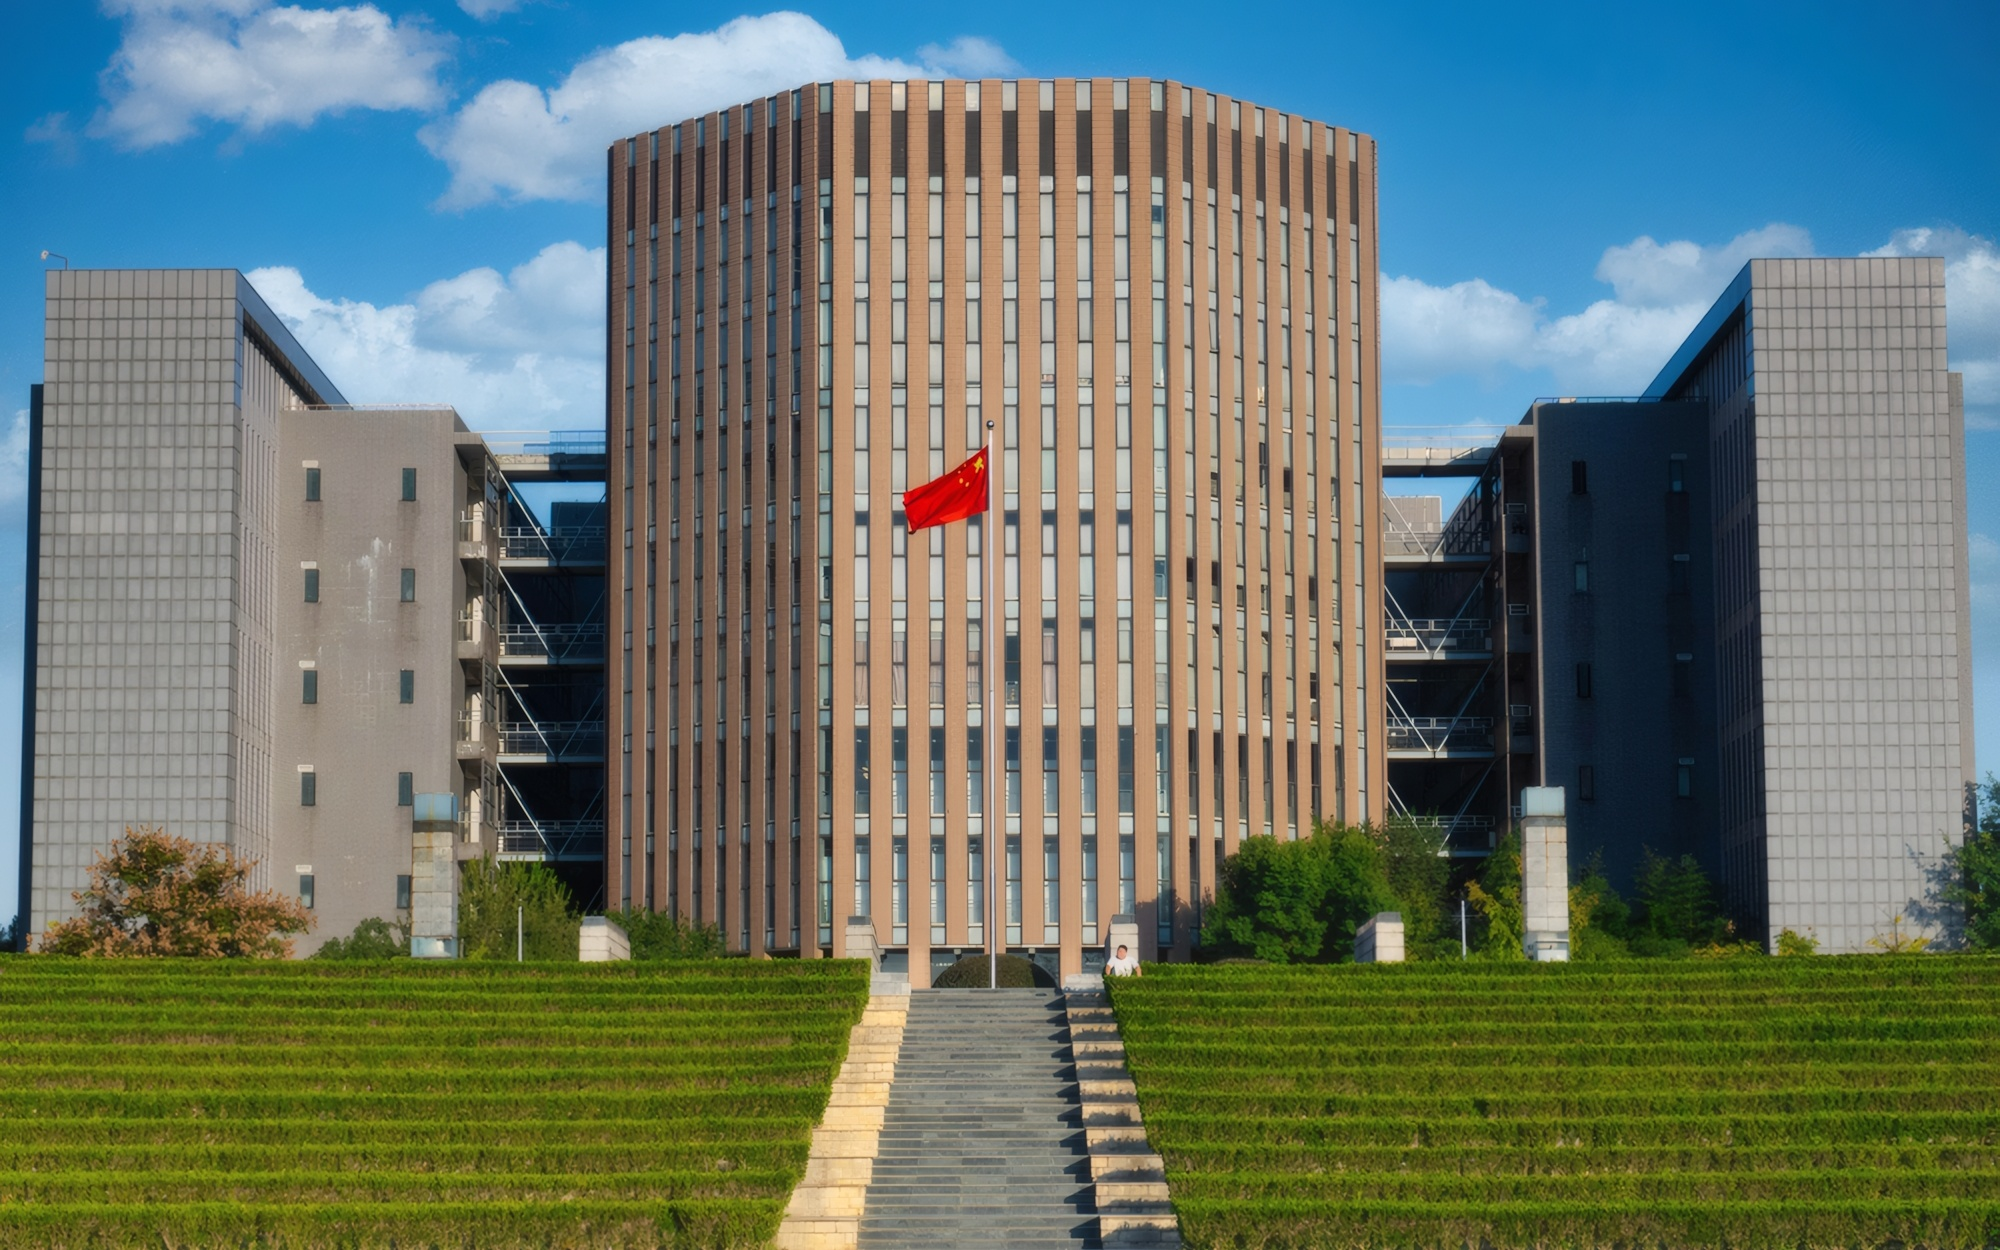
\includegraphics[height=2.3cm]{src/example_ahu.jpg}\label{fig:campus-a}}
\hspace{0.5cm}
\subfloat[校园风光]{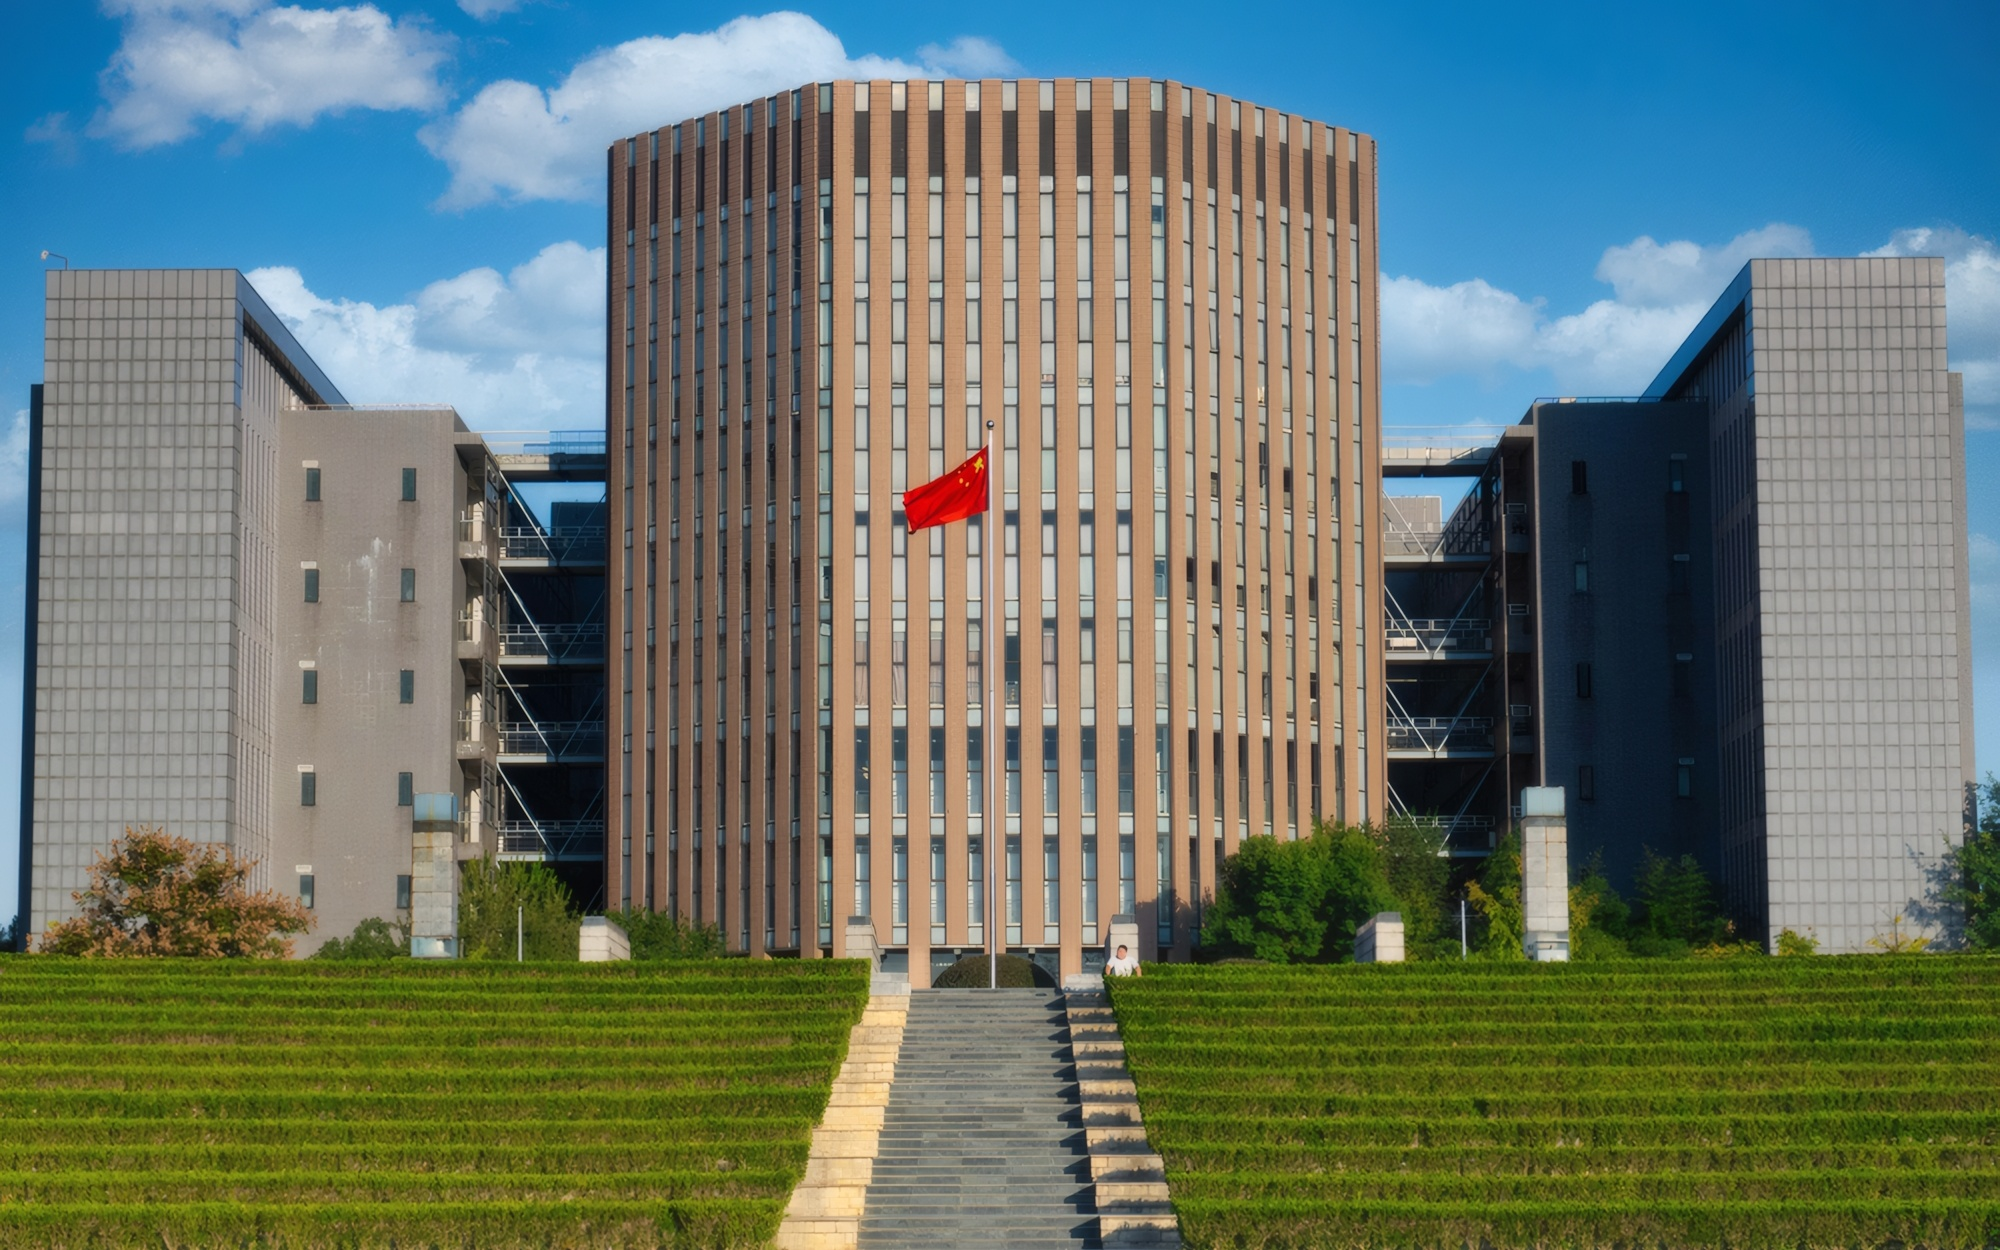
\includegraphics[height=2.3cm]{src/example_ahu.jpg}\label{fig:campus-b}}
\caption{安徽大学磬苑校区景观示例（子图编号自动生成）}
\label{fig:campus}
\end{figure}

\vspace{-0.3em}
\begin{block}{说明}
使用 \texttt{subfig} 宏包的 \texttt{subfloat} 命令实现子图并排，
每个子图可独立添加标签和标题，方便在正文中引用，如图~\ref{fig:campus-a} 和图~\ref{fig:campus-b}。
\end{block}
\end{frame}
